\section{Experiments}
\label{sec:experiments}
\begin{figure*}
	\centering
	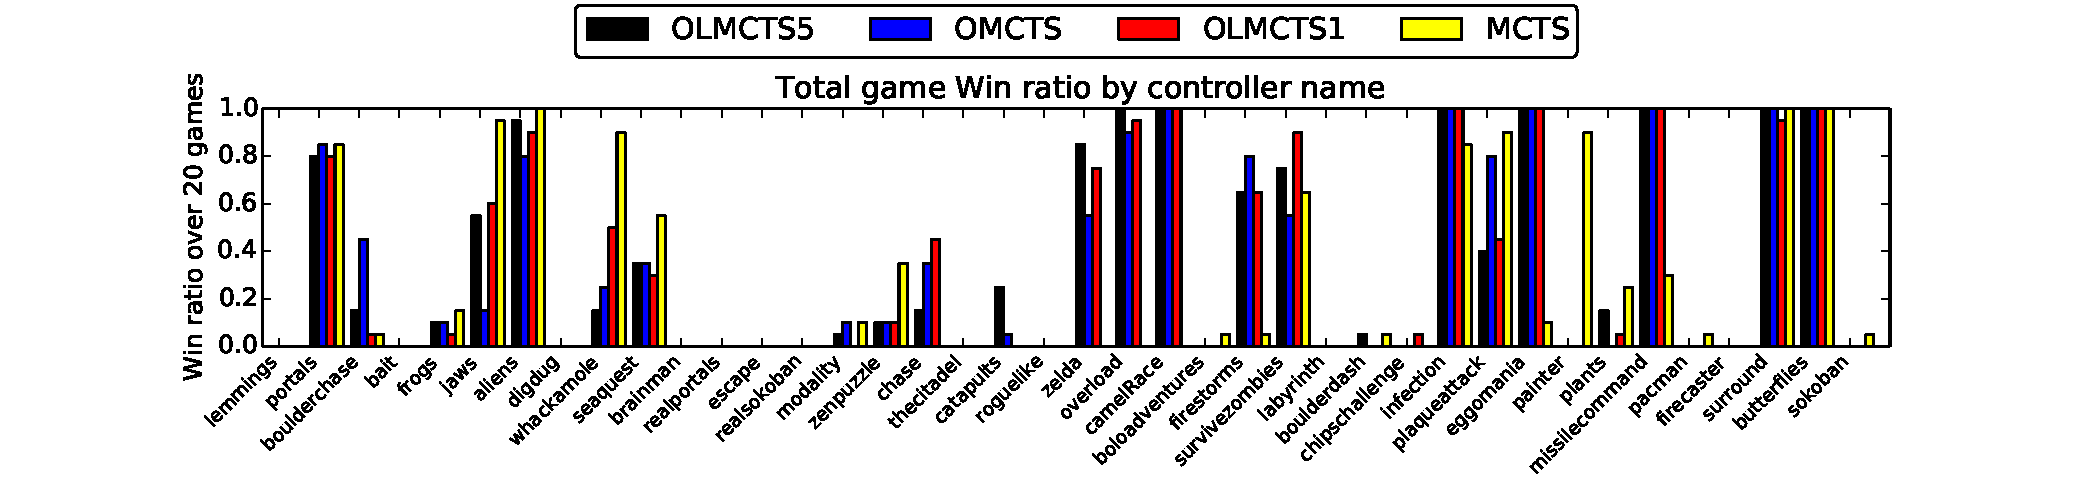
\includegraphics[width=\textwidth]{includes/wins}
	\vspace{-.8cm}
	\caption{Win ratio of the algorithms per game on all levels.}
	\label{fig:wins}
\end{figure*}

\begin{figure*}
	\centering
	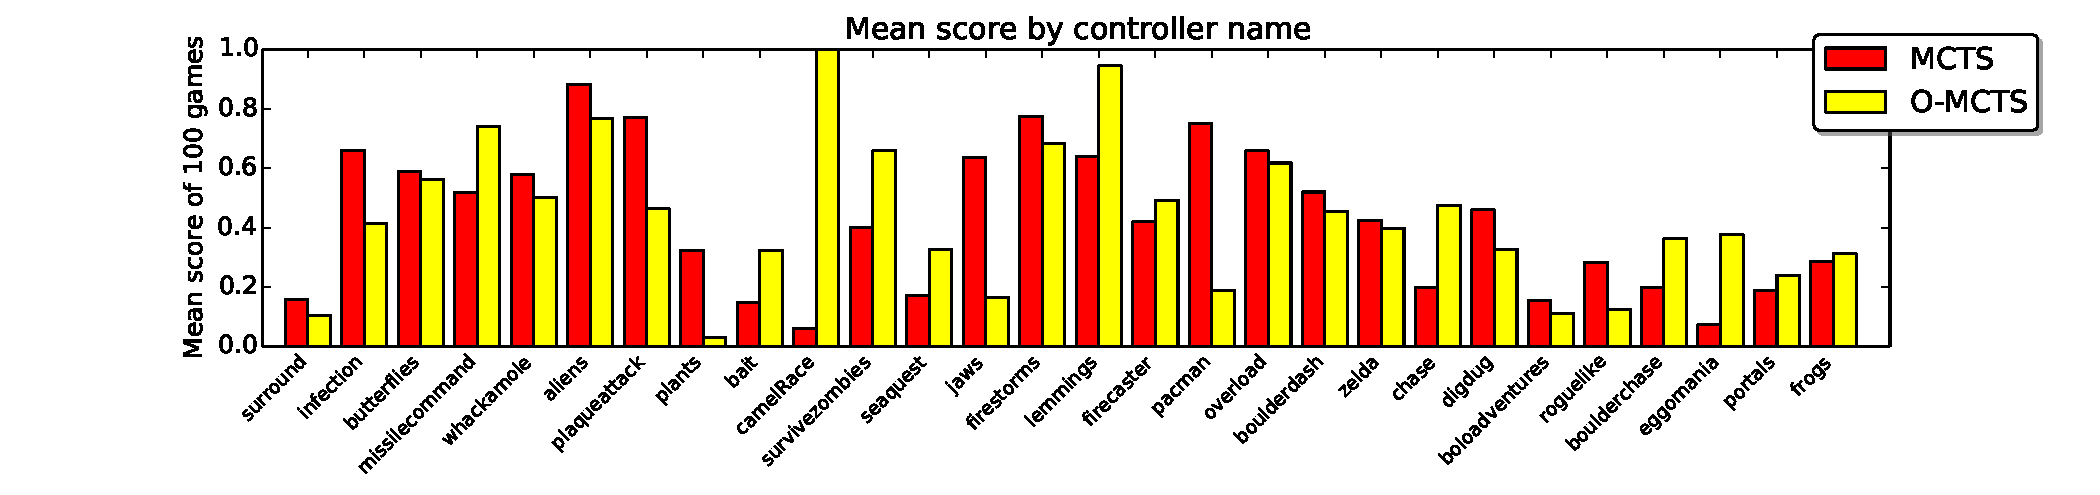
\includegraphics[width=\textwidth]{includes/scores}
	\vspace{-.8cm}
	\caption{Normalized mean score of the algorithms per game 1 means the
	highest score achieved by all the algoriths, 0 the lowest.}
	\label{fig:scores}
\end{figure*}
\begin{figure}
	\centering
	\subfigure[Learning \textit{bait}]{
		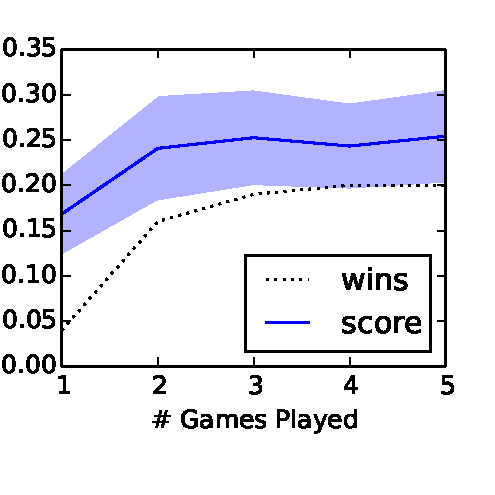
\includegraphics[scale=.44]{includes/learning}
		\label{fig:learning-results}
	}
	\subfigure[Totals]{
		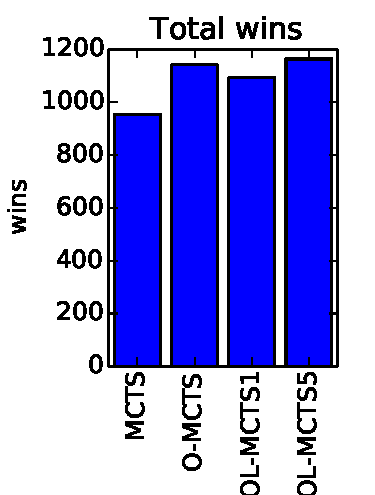
\includegraphics[scale=.44]{includes/totals.pdf}
		\label{fig:learning-results}
	}
	\caption{Learning improvement and total number of wins of the algorithms on
	all games}
\end{figure}

In this section we compare O-MCTS and OL-MCTS to traditional MCTS by running
simulations on 40 different games in the VGDL framework. For this experiment
we constructed the following option types. More options can be created and added
to the algorithm easily.

\begin{itemize}[noitemsep]
	\item \texttt{ActionOption} executes a specific action once and then
		stops.
	\item \texttt{AvoidNearestNpcOption} makes the agent avoid the nearest NPC
	\item \texttt{GoNearMovableOption} makes the agent walk towards a
		movable game sprite and stops when it is within a certain range of the
		movable
	\item \texttt{GoToMovableOption} makes the agent walk towards a
		movable until its location is the same as that of the movable
	\item \texttt{GoToNearestSpriteOfType} makes the agent walk to the nearest sprite of
		a specific type
	\item \texttt{GoToPositionOption} makes the agent walk to a specific position
	\item \texttt{WaitAndShootOption} waits until an NPC is in a specific location and
		then uses its weapon.
\end{itemize}

For each option type, a subtype per game sprite is created during the game. For
each sprite, an option of the corresponding subtype is created. For example, the
game Zelda contains three different sprite types (excluding the avatar); a
monster, a key and a portal. The first level contains three monsters, one key
and one portal and the aim of the game is to collect the key and walk towards
the portal without walking into the monsters. In the first level, there are
three monsters, one key and one portal. \texttt{GoToMovableOption} and
\texttt{GoNearMovableOptions} will be created for each of the three monsters and
for the key. A \texttt{GoToPositionOption} will be created for the portal.
One \texttt{GoToNearestSpriteOfType} will be created per sprite type. One
\texttt{WaitAndShootOption} will be created for the monsters, and one
\texttt{AvoidNearestNpcOption} will be
created. This set of options is $O$ in algorithms \ref{alg:omcts} and
\ref{alg:olmcts}.

Furthermore, in these experiments we use discount factor $\gamma = 0.9$,
maximum action time $t = 40$ milliseconds. The maximum search depth $d$
is set to 80, which is higher than most tree search algorithms use in GVGAI. The
number of node visits $v$ is set to 40, after which \textsf{uct} is used. $K$
for crazy stone is set to $0.5$.

For comparison, we use the MCTS algorithm provided with the Java implementation
of VGDL with its default value of maximum search depth 8. 

We ran the algorithms on a set of 40 different games with 5 levels each. For
each level, we use the mean results of 20 plays. For the transfer learning
algorithm the fifth game after 4 training games was used (it played 100
games per level altogether).

Figures \ref{fig:wins} and \ref{fig:scores} respectively show the win ratio and
normalized score for each game and algorithm.
